\section{Folgen und Reihen}\label{sec:folgen-und-reihen}

\begin{definition}{Definition}
    Eine reelle \emph{Folge} $a$ ist eine Funktion (Abbildung) $a : \N^* \rightarrow \R$, die jeder natürlichen Zahl $n \in \N^*$ eine reelle Zahl $a_n$ zuordnet.

    Indexnotation: $a_n$ ist das $n-te$ Glied der Folge $a$.\\
    Schreibweise: $a = (a_n)$ (oder auch $a = \langle a_n \rangle$).

    Bei einer Folge haben wir es mit unendlich vielen Objekten (reellen Zahlen) zu tun.
\end{definition}

\begin{definition}{Arithmetische Folge}
    Mit $c,d \in \R$
    \begin{itemize}
        \item \textbf{Aufzählende Darstellung:} $c, c + d, c + 2d, c + 3d, \dots$
        \item \textbf{Explizite Darstellung:} $a_n = c + (n - 1)d$
        \item \textbf{Implizite Darstellung:} $a_1 = c$ und $a_{n+1} = a_n + d$
    \end{itemize}
\end{definition}

\begin{definition}{Geometrische Folge}
    Mit $c, q \in \R$ und $q \neq 0,1$
    \begin{itemize}
        \item \textbf{Aufzählende Darstellung:} $c, c \cdot q, c \cdot q^2, c \cdot q^3, \dots$
        \item \textbf{Explizite Darstellung:} $a_n = c \cdot q^{n-1}$
        \item \textbf{Implizite Darstellung:} $a_1 = c$ und $a_{n+1} = a_n \cdot q$
    \end{itemize}
\end{definition}

\begin{definition}{Harmonische Folge}
    \begin{itemize}
        \item \textbf{Aufzählende Darstellung:} $1, \frac{1}{2}, \frac{1}{3}, \frac{1}{4}, \dots$
        \item \textbf{Explizite Darstellung:} $a_n = \frac{1}{n}$
        \item \textbf{Implizite Darstellung:} (Nicht üblich)
    \end{itemize}
\end{definition}

\begin{definition}{Fibonacci-Folge}
    \begin{itemize}
        \item \textbf{Aufzählende Darstellung:} $1, 1, 2, 3, 5, 8, 13, 21, \dots$
        \item \textbf{Explizite Darstellung:} (Nicht elementar)
        \item \textbf{Implizite Darstellung:} $a_1 = 1$, $a_2 = 1$ und $a_{n+2} = a_n + a_{n+1}$
    \end{itemize}
\end{definition}

\subsection{Grenzwerte von Folgen}\label{subsec:grenzwerte-von-folgen}

\begin{definition}{Definition}
    Eine reelle Zahl $g$ heisst \emph{Grenzwert} oder \emph{Limes} der Folge $a_n$, wenn es zu jedem $\epsilon > 0$ eine natürliche Zahl $n_0$ gibt, sodass für alle $n \geq n_0$ stets $|a_n - g| < \epsilon$ gilt.
    Eine Folge heisst \emph{konvergent}, wenn sie einen Grenzwert $g$ hat.
\end{definition}

\begin{center}
    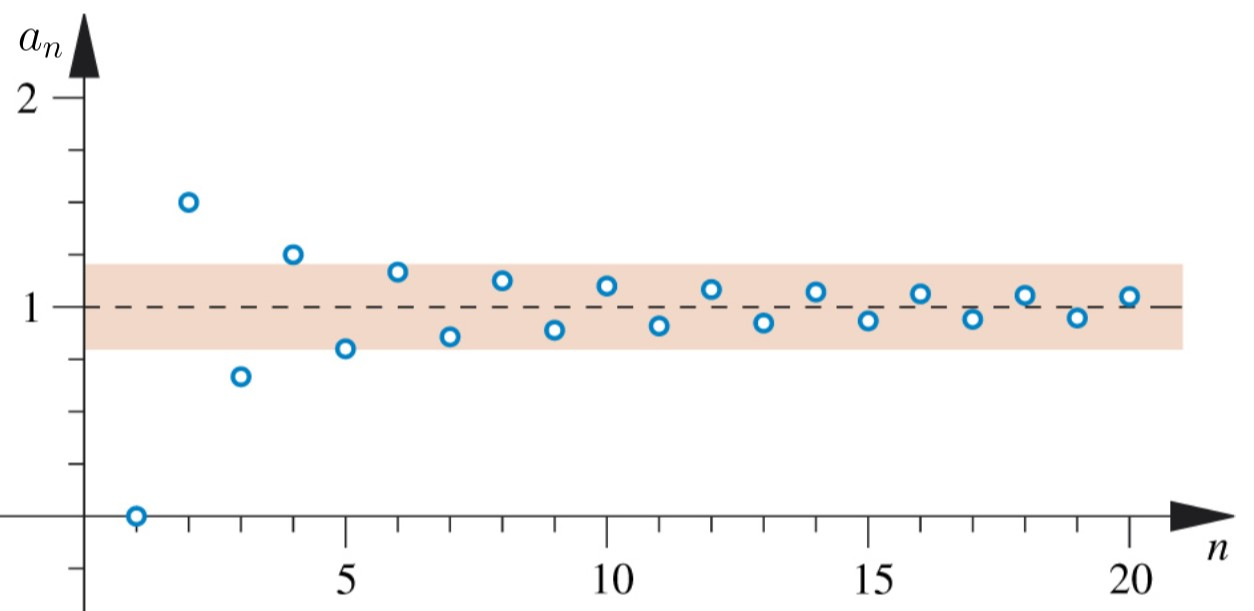
\includegraphics[scale=0.27]{limes}
\end{center}

Damit man sicher sein kann, dass die Punkte immer näher an den geforderten Wert kommen, muss man die Breite des betrachteten Streifens beliebig klein wählen dürfen.
Die Formel dazu lautet: \[g - \epsilon < a_n < g + \epsilon \quad \text{resp.} \quad |a_n - g| < \epsilon\]
Schreibweise: $\lim \limits_{n \rightarrow \infty} a_n = g$.

Eine Folge $a_n$, die keinen Grenzwert hat, heisst \emph{divergent}.

\textbf{Bemerkung:} Eine Folge hat höchstens einen Grenzwert.

\begin{definition}{Rechenregeln für Grenzwerte}
    Gegeben sind zwei konvergente Folgen $a$ und $b$ und eine Konstant $c$.
    Dann gelten:
    \begin{enumerate}
        \item $\lim \limits_{n \rightarrow \infty} (c \cdot a_n) = c \cdot \lim \limits_{n \rightarrow \infty} a_n$
        \item $\lim \limits_{n \rightarrow \infty} (a_n + b_n) = \lim \limits_{n \rightarrow \infty} a_n + \lim \limits_{n \rightarrow \infty} b_n$
        \item $\lim \limits_{n \rightarrow \infty} (a_n - b_n) = \lim \limits_{n \rightarrow \infty} a_n - \lim \limits_{n \rightarrow \infty} b_n$
        \item $\lim \limits_{n \rightarrow \infty} (a_n \cdot b_n) = \lim \limits_{n \rightarrow \infty} a_n \cdot \lim \limits_{n \rightarrow \infty} b_n$
        \item $\lim \limits_{n \rightarrow \infty} \frac{a_n}{b_n} = \frac{\lim \limits_{n \rightarrow \infty} a_n}{\lim \limits_{n \rightarrow \infty} b_n}$, falls $\lim \limits_{n \rightarrow \infty} b_n \neq 0$ und $b_n \neq 0$ für alle $n$.
    \end{enumerate}
\end{definition}

\textbf{Bemerkung:} Wir betrachten eine Folge $a$, die eine rationale Funktion ist, d.h.\ die Folgenglieder sind von der Form $a_n = \frac{g(n)}{h(n)}$, wobei $g(n)$ und $h(n)$ Polynome sind.
Dann wird der Grenzwert $\lim \limits_{n \rightarrow \infty} a_n$ so bestimmt:
\begin{enumerate}
    \item Der Bruch wird mit der höchsten Potenz von $n$, die vorkommt, gekürzt.
    \item Nun wird das Verhalten der einzelnen Summanden für $n \rightarrow \infty$ untersucht.
    \item Daraus kann man den gesuchten Grenzwert bestimmen.
\end{enumerate}
\textbf{Folgerung:} Um den Grenzwert für $n \rightarrow \infty$ zu bestimmen, reicht es, den \emph{höchsten} Exponenten im Zähler und den höchsten Exponenten im Nenner zu betrachten.
Es gibt drei mögliche Fälle:
\begin{itemize}
    \item[] \textbf{Fall 1:} Zählergrad $<$ Nennergrad.
    Dann gilt: $\lim \limits_{n \rightarrow \infty} \frac{g(n)}{h(n)} = 0$\\
    Beispiel: $\lim \limits_{n \rightarrow \infty} \frac{3n^2 + 7n - 15}{n^3 - 2n^2 + n + 10} = 0$
    \item[] \textbf{Fall 2:} Zählergrad $>$ Nennergrad.
    Dann gilt: $\frac{g(n)}{h(n)} \rightarrow \infty$ oder ($-\infty$)\\
    Beispiel: $\frac{3n^4 + 7n - 15}{6n^3 - 2n^2 + 10} \rightarrow \infty$
    \item[] \textbf{Fall 3:} Zählergrad $=$ Nennergrad.
    Dann gilt: $\lim \limits_{n \rightarrow \infty} \frac{g(n)}{h(n)} = \frac{\text{``Führender Term von $g$''}}{\text{``Führender Term von $h$''}}$\\
    Beispiel: $\lim \limits_{n \rightarrow \infty} \frac{2n^3 + n^2 + 8n}{5n^3 + 4n^2 + 17} = \frac{2}{5}$
\end{itemize}

\textbf{Bemerkung:} Die spezielle Folge $\langle \left(1 + \frac{1}{n}\right)^n \rangle$ strebt gegen $e \approx 2.718$.

\subsection{Reihen - einige besondere Beispiele}\label{subsec:reihen-beispiele}

\begin{definition}{Definition}
    Die \emph{Summenfolge} oder \emph{Reihe} $s$ der reelle Folge $a$ ist definiert durch:
    \begin{align*}
        s_1 &= a_1 \\
        s_2 &= a_1 + a_2 \\
        s_3 &= a_1 + a_2 + a_3 \\
        &\vdots \\
        s_n &= a_1 + a_2 + \dots + a_n = \sum \limits_{k=1}^n a_k
    \end{align*}
    Auch ``$n$-te Teilsumme'' genannt.
\end{definition}

\begin{definition}{Arithmetische Reihe}
    Bei einer \emph{arithmetischen Folge} ist die Differenz zweier aufeinanderfolgender Glieder konstant:\\ $a_k - a_{k-1} = d$ für jedes $k$.
    Die Summe der ersten $n$ Glieder einer arithmetischen Folge ist: \[s_n = n \cdot a_1 + \frac{n(n-1)}{2} \cdot d\]
\end{definition}

\begin{definition}{Geometrische Reihe}
    Bei einer \emph{geometrischen Folge} ist der Quotient zweier aufeinanderfolgender Glieder konstant:\\ $\frac{a_k}{a_{k-1}} = q$ für jedes $k$ (mit $q \neq 0, 1$).
    Die Summe der ersten $n$ Elemente einer geometrischen Reihe ist: \[s_n = \frac{a_1 (q^n - 1)}{q - 1} = \frac{a_1 (1 - q^n)}{1 - q}\]
\end{definition}

\subsection{Grenzwerte von Reihen}\label{subsec:grenzwerte-reihen}

Für den Grenzwert der Reihe $s$ einer reellen Folge $a$ schreiben wir: $g = \lim \limits_{n \rightarrow \infty} s_n = \sum_{k=1}^\infty a_k$

% TODO: Andere Reihen auflisten

\textbf{Allgemein (Geometrische Reihe):} Wie verhält sich $s_n = a_1 \cdot \frac{1-q^n}{1-q}$, wenn $n \rightarrow \infty$?
\begin{itemize}
    \item[] \textbf{Fall 1:} $q > 1$.
    Die Reihe strebt gegen $\infty$ oder $-\infty \rightarrow$ Sie hat keinen Grenzwert.
    \item[] \textbf{Fall 2:} $q \leq -1$.
    Die Reihe sprint zwischen positiven und negativen Werten hin und her $\rightarrow$ Sie hat keinen Grenzwert.
    \item[] \textbf{Fall 3:} $|q| < 1$.
    Die Reihe strebt gegen den Grenzwert $a_1 \cdot \frac{1}{1-q}$.
\end{itemize}

\begin{definition}{Zusammenfassung}
    Eine geometrische Reihe konvergiert genau dann, wenn $|q| < 1$ ist.
    Der Grenzwert ist dann $\frac{a_1}{1-q}$.
\end{definition}